% =============================================================================
% Chapter 4: SLAM and Mapping with Thermal-Visual Fusion
% =============================================================================
\selectlanguage{hebrew}

\section{מיפוי ומיקום סימולטני עם מיזוג תרמי-חזותי}
\label{sec:ch04_slam}

\subsection{מבוא לבעיית ה-SLAM בסביבות לילה}
\label{sec:ch04_intro}

בעיית המיפוי והמיקום הסימולטני (\en{Simultaneous Localization and Mapping, SLAM}) מהווה את אחת הבעיות היסודיות ביותר ברובוטיקה אוטונומית. היכולת של רחפן לנווט בסביבה לא מוכרת תוך בנייה בו-זמנית של מפת הסביבה ואומדן מיקומו בתוכה היא תנאי הכרחי לפעולה אוטונומית מלאה. בעוד שמערכות \en{SLAM} חזותיות מבוססות מצלמת \en{RGB} הציגו ביצועים מרשימים בתנאי תאורה טובים, כפי שהודגם במערכות \en{ORB-SLAM3} \cite{Campos2021ORBSLAM3} ו-\en{VINS-Mono} \cite{Qin2018VINSMono}, ביצועיהן יורדים דרמטית בתנאי תאורה נמוכה, בהם זיהוי והתאמת נקודות עניין הופכים לבלתי אמינים.

השילוב של מצלמה תרמית במסגרת \en{SLAM} מציע פתרון טבעי לאתגר זה. מצלמה תרמית פועלת בתחום הספקטרלי של 8-14 $\mu$m, בו קרינת גוף שחור של עצמים בטמפרטורת הסביבה (250-320 K) מספקת ניגודיות תמונה גם בהיעדר מוחלט של תאורה חיצונית. עם זאת, תמונות תרמיות סובלות מרעש גבוה יותר, רזולוציה מרחבית נמוכה יותר, והיעדר מרקם חזותי עשיר האופייני לתמונות \en{RGB}. אתגרים אלה מחייבים פיתוח שיטות עיבוד ייחודיות המותאמות לאופי המיוחד של התמונה התרמית.

בפרק זה אנו מציגים מסגרת \en{SLAM} היברידית המשלבת מידע ממצלמה תרמית וממצלמה חזותית. המסגרת מבוססת על ארכיטקטורת גרף-\en{SLAM} עם אופטימיזציית \en{pose graph} תוך שימוש באילוצים משתי המודאליות. אנו מציגים שיטה חדשה להתאמת נקודות עניין בין תמונות תרמיות לחזותיות, המבוססת על למידה עמוקה של תכונות מודאליות-חוצות. בנוסף, אנו מציגים מנגנון להערכת עומק ממצלמה תרמית יחידה המנצל את הקשר בין עוצמת הקרינה התרמית למרחק.

\subsection{יסודות תורתיים של SLAM מבוסס גרף}
\label{sec:ch04_graph_slam}

מסגרת ה-\en{SLAM} המוצעת מבוססת על גישת גרף-\en{SLAM} (\en{Graph-SLAM}), המיוצגת כגרף פקטורים (\en{factor graph}) שבו צמתים מייצגים משתני מצב (מיקומי רחפן ומיקומי נקודות ציון), וקשתות מייצגות אילוצים הנובעים מתצפיות חיישנים ומדידות אודומטריה. האופטימיזציה מתבצעת על ידי מזעור פונקציית עלות לוג-סבירות שלילית באמצעות אופטימיזציית ריבועים קטנים לא-לינארית דלילה \cite{Grisetti2010g2o, Kaess2012iSAM2}.

פונקציית העות הכוללת מוגדרת כסכום של אילוצים מכל המודאליות:

\begin{equation}
\mathcal{E}_{\text{total}} = \sum_{(i,j) \in \mathcal{V}} \r$h$o_$h(\mathbf{e}_{ij}^T \mathbf{\Omega}_{ij} \mathbf{e}_{ij})$$$ + \sum_{(i,j) \in \mathcal{T}} \r$h$o_$h(\mathbf{e}_{ij}^{\text{therm},T} \mathbf{\Omega}_{ij}^{\text{therm}} \mathbf{e}_{ij}^{\text{therm}})$$$ + \sum_{(i,j) \in \mathcal{L}} \r$h$o_$h(\mathbf{e}_{ij}^{\text{loop},T} \mathbf{\Omega}_{ij}^{\text{loop}} \mathbf{e}_{ij}^{\text{loop}})$$$
\label{eq:ch04_total_cost}
\end{equation}

כאשר $\mathcal{V}$, $\mathcal{T}$, ו-$\mathcal{L}$ מייצגים את קבוצות האילוצים החזותיים, התרמיים, וסגירת הלולאה בהתאמה. $\rho_h$ היא פונקציית המחיר החסינה של \en{Huber} המפחיתה את השפעתם של חריגים (\en{outliers}). $\mathbf{e}_{ij}$ הוא וקטור שגיאת הריבוי (\en{reprojection error}) עבור תצפית $j$ ממיקום $i$, ו-$\mathbf{\Omega}_{ij}$ היא מטריצת המידע (הופכי מטריצת השונות) המשויכת לתצפית.

שגיאת הריבוי עבור תצפית חזותית מוגדרת כ:

\begin{equation}
\mathbf{e}_{ij}^{\text{vis}} = \mathbf{z}_{ij}^{\text{vis}} - \pi_{\text{vis}}(\mathbf{T}_{cw} \cdot \mathbf{X}_j)
\label{eq:ch04_reprojection_vis}
\end{equation}

כאשר $\mathbf{z}_{ij}^{\text{vis}} \in \mathbb{R}^2$ היא נקודת התמונה הנצפית במצלמה החזותית, $\pi_{\text{vis}}: \mathbb{R}^3 \to \mathbb{R}^2$ היא פונקציית ההטלה של המצלמה החזותית, $\mathbf{T}_{cw} \in SE(3)$ היא טרנספורמציית היציבה בין מערכת הקואורדינטות העולמית למערכת המצלמה, ו-$\mathbf{X}_j \in \mathbb{R}^3$ היא נקודת הציון התלת-ממדית.

באופן אנלוגי, שגיאת הריבוי עבור תצפית תרמית מוגדרת כ:

\begin{equation}
\mathbf{e}_{ij}^{\text{therm}} = \mathbf{z}_{ij}^{\text{therm}} - \pi_{\text{therm}}(\mathbf{T}_{cw}^{\text{therm}} \cdot \mathbf{X}_j)
\label{eq:ch04_reprojection_therm}
\end{equation}

כאשר $\pi_{\text{therm}}$ היא פונקציית ההטלה של המצלמה התרמית, ו-$\mathbf{T}_{cw}^{\text{therm}}$ היא טרנספורמציית היציבה ביחס למצלמה התרמית, המקושרת ל-$\mathbf{T}_{cw}$ באמצעות כיול חיצוני (\en{extrinsic calibration}) בין שתי המצלמות.

\subsection{התאמת נקודות עניין בין-מודאלית}
\label{sec:ch04_cross_modal_matching}

אחד האתגרים המרכזיים בשילוב מצלמה תרמית במסגרת \en{SLAM} הוא התאמת נקודות עניין בין תמונות תרמיות לחזותיות. שיטות התאמה מסורתיות המבוססות על תכונות גיאומטריות מקומיות (\en{SIFT}, \en{ORB}) נכשלות כאשר המודאליות שונה, שכן המראה החזותי של אותה נקודה פיזיקלית שונה מהותית בין הספקטרום הנראה לתת-אדום.

כדי להתגבר על אתגר זה, אנו מציעים שיטת התאמה מבוססת למידה עמוקה המשתמשת ברשת סיאמית (\en{Siamese network}) ללימוד תכונות מודאליות-חוצות. הרשת מורכבת משני ענפים זהים, האחד מעבד תמונות חזותיות והשני תמונות תרמיות, כאשר המשקולות משותפות בין הענפים. כל ענף מייצר וקטור תכונה באורך 128 ממדים עבור כל נקודת עניין.

מרחק ההתאמה בין נקודת עניין חזותית $i$ לנקודת עניין תרמית $j$ מוגדר כ:

\begin{equation}
d_{ij} = \| \mathbf{f}_{\text{vis}}(\mathbf{p}_i) - \mathbf{f}_{\text{therm}}(\mathbf{p}_j) \|_2
\label{eq:ch04_feature_distance}
\end{equation}

כאשר $\mathbf{f}_{\text{vis}}$ ו-$\mathbf{f}_{\text{therm}}$ הם פונקציות מיצוי התכונות מהרשת הסיאמית. התאמה מתקבלת כאשר $d_{ij} < \tau$ וההתאמה היא הדדית (\en{mutual nearest neighbor}).

הרשת מאומנת על מערך נתונים של זוגות תמונות חזותיות-תרמיות מיושרות, תוך שימוש בפונקציית ההפסד הבאה:

\begin{equation}
\mathcal{L}_{\text{match}} = \sum_{(i,j) \in \mathcal{P}} d_{ij}^2 + \sum_{(i,k) \in \mathcal{N}} \m$a$x(0, m - d_{ik})$$^2
\label{eq:ch04_contrastive_loss}
\end{equation}

כאשר $\mathcal{P}$ היא קבוצת זוגות תואמים (\en{positive pairs}), $\mathcal{N}$ היא קבוצת זוגות שאינם תואמים (\en{negative pairs}), ו-$m$ הוא מרווח (\en{margin}) שנקבע כ-$m = 1.0$ בניסויים שלנו.

\subsection{אומדן עומק ממצלמה תרמית יחידה}
\label{sec:ch04_depth_estimation}

אתגר משמעותי נוסף בשימוש במצלמה תרמית יחידה ל-\en{SLAM} הוא היעדר מידע עומק ישיר. בעוד שמצלמת \en{RGB} יכולה להסתמך על משולשות (\en{triangulation}) מתנועה (\en{Structure from Motion, SfM}) או ממצלמת סטריאו, התמונה התרמית מציבה אתגרים ייחודיים בשל הרזולוציה הנמוכה והרעש הגבוה.

אנו מציעים שיטה להערכת עומק יחסי מתמונה תרמית יחידה המבוססת על הקשר בין עוצמת הקרינה התרמית הנקלטת למרחק. על פי חוק סטפן-בולצמן, עוצמת הקרינה הנקלטת במצלמה תרמית מעצם במרחק $d$ נתונה על ידי:

\begin{equation}
I_{\text{therm}}(\mathbf{p}) = \frac{\epsilon(\mathbf{p}) \sigma T(\mathbf{p})^4}{\pi} \cdot \tau_{\text{atm}}(d) \cdot \frac{A_{\text{lens}}}{d^2} + I_{\text{path}}(d)
\label{eq:ch04_thermal_radiation}
\end{equation}

כאשר $\epsilon$ היא פליטות העצם, $\sigma$ הוא קבוע סטפן-בולצמן, $T$ היא טמפרטורת העצם, $\tau_{\text{atm}}$ היא העברת האטמוספירה, $A_{\text{lens}}$ היא שטח העדשה, ו-$I_{\text{path}}$ היא קרינת הנתיב האטמוספירי.

בהנחה שטמפרטורת העצם קבועה לאורך זמן קצר, השינוי בעוצמה הנקלטת נובע בעיקר משינוי במרחק. ניתן לבצע ליניאריזציה של הקשר באמצעות קירוב מסדר ראשון:

\begin{equation}
\Delta I_{\text{therm}} \approx -\frac{2I_0}{d_0} \Delta d + \frac{\partial I_{\text{path}}}{\partial d} \Delta d
\label{eq:ch04_depth_linearization}
\end{equation}

כאשר $I_0$ היא העוצמה הנקלטת במרחק הייחוס $d_0$. קשר זה מאפשר הערכת שינוי עומק יחסי מתצפיות תרמיות עוקבות, ומשמש כאילוץ נוסף באופטימיזציית הגרף.

\subsection{SLAM תרמי-חזותי מבוסס גרף}
\label{sec:ch04_graph_thermal_visual}

המסגרת המשולבת שלנו משלבת את כל הרכיבים שתוארו לעיל לתוך מערכת \en{SLAM} מאוחדת. הארכיטקטורה מבוססת על שלושה חוטי עיבוד מקבילים: חוט מעקב (\en{tracking thread}) הפועל בזמן אמת בקצב של 30 הרץ, חוט מיפוי מקומי (\en{local mapping thread}) הפועל בקצב של 5 הרץ, וחוט סגירת לולאה (\en{loop closing thread}) הפועל בקצב מופחת.

חוט המעקב מבצע את השלבים הבאים בכל פריים:

\begin{enumerate}
  \item רכישת תמונה חזותית ותרמית בו-זמנית
  \item חילוץ נקודות עניין משתי התמונות באמצעות רשת סיאמית מאומנת
  \item התאמת נקודות עניין בין הפריים הנוכחי לפריים המפתח האחרון
  \item אומדן ראשוני של היציבה באמצעות אופטימיזציית \en{motion-only BA}
  \item עדכון מפת נקודות הציון המקומית
\end{enumerate}

אופטימיזציית היציבה (\en{motion-only BA}) מנסחת את הבעיה כמזעור של שגיאת הריבוי המשוקללת משתי המודאליות:

\begin{equation}
\{ \mathbf{R}, \mathbf{t} \}^* = \arg\min_{\mathbf{R}, \mathbf{t}} \l$e$f$t( \sum_{i \in \mathcal{V}} \r$h$o_$h( \| \pi_{\text{vis}}(\mathbf{R} \mathbf{X}_i + \mathbf{t})$$$$$$ - \mathbf{x}_i^{\text{vis}} \|_{\Sigma_i}^2 ) + \lambda \sum_{j \in \mathcal{T}} \r$h$o_$h( \| \pi_{\text{therm}}(\mathbf{R} \mathbf{X}_j + \mathbf{t})$$$ - \mathbf{x}_j^{\text{therm}} \|_{\Sigma_j}^2 ) \right)
\label{eq:ch04_motion_ba}
\end{equation}

כאשר $\lambda$ הוא מקדם איזון בין המודאליות, הנקבע באופן אדפטיבי בהתאם לאיכות ההתאמה בכל מודאליות. כאשר תנאי התאורה טובים, $\lambda < 1$ והמודאליות החזותית מקבלת משקל גבוה יותר. בתנאי חושך, $\lambda > 1$ והמודאליות התרמית הופכת לדומיננטית.

\subsection{סגירת לולאה ואופטימיזציית גרף גלובלית}
\label{sec:ch04_loop_closure}

זיהוי סגירת לולאה (\en{loop closure detection}) הוא מרכיב קריטי במערכת \en{SLAM} המאפשר תיקון סחיפה מצטברת. המערכת שלנו משתמשת בשיטה היברידית המשלבת זיהוי מבוסס \en{bag-of-words} (\en{DBoW2}) עם זיהוי מבוסס תכונות תרמיות-חזותיות.

כאשר מתגלה סגירת לולאה פוטנציאלית, מתבצע אימות גיאומטרי באמצעות אלגוריתם \en{RANSAC} עם אומדן \en{Sim(3)} ליישור המפות. אילוץ סגירת הלולאה מתווסף לגרף הפקטורים:

\begin{equation}
\mathbf{e}_{ij}^{\text{loop}} = \mathbf{T}_{ij}^{\text{loop}} \ominus (\mathbf{T}_{iw} \ominus \mathbf{T}_{jw})
\label{eq:ch04_loop_constraint}
\end{equation}

כאשר $\mathbf{T}_{ij}^{\text{loop}}$ היא טרנספורמציית היציבה היחסית שהוערכה מסגירת הלולאה, ו-$\mathbf{T}_{iw}$ ו-$\mathbf{T}_{jw}$ הן יציבות הצמתים $i$ ו-$j$ במערכת הקואורדינטות העולמית. האופרטור $\ominus$ מייצג את ההפרש במרחב $SE(3)$.

לאחר הוספת אילוץ סגירת הלולאה, מתבצעת אופטימיזציית גרף גלובלית באמצעות אלגוריתם \en{Gauss-Newton} עם מטריצת יאקובי דלילה:

\begin{equation}
(\mathbf{J}^T \mathbf{\Omega} \mathbf{J}) \Delta \mathbf{x} = -\mathbf{J}^T \mathbf{\Omega} \mathbf{e}
\label{eq:ch04_gn_step}
\end{equation}

כאשר $\mathbf{J}$ היא מטריצת היאקובי של כל אילוצי השגיאה, $\mathbf{\Omega}$ היא מטריצת המידע המשולבת, $\Delta \mathbf{x}$ הוא עדכון המשתנים, ו-$\mathbf{e}$ הוא וקטור השגיאות הכולל.

\subsection{ניתוח דיוק ועמידות}
\label{sec:ch04_analysis}

כדי להעריך את ביצועי מערכת ה-\en{SLAM} המוצעת, ערכנו סדרת ניסויים על מערך נתונים לילי שאספנו. מערך הנתונים כולל מסלולים באורך כולל של 5.2 ק"מ בסביבות עירוניות וטבעיות בתנאי תאורה משתנים (0.01-100 לוקס).

\begin{table}[htbp]
\centering
\caption{השוואת ביצועי SLAM בתנאי תאורה שונים. (SLAM performance comparison under varying illumination conditions.)}
\label{tab:ch04_slam_results}
\adjustbox{max width=\columnwidth}{%
\begin{tabular}{lcccc}
\toprule
\textbf{שיטה} & \textbf{תאורה [lux]} & \textbf{ATE [m]} & \textbf{RPE [m/s]} & \textbf{הצלחה [\%]} \\
\midrule
ORB-SLAM3 (חזותי בלבד) & $>50$ & 0.12 & 0.04 & 98 \\
ORB-SLAM3 (חזותי בלבד) & 1-50 & 0.45 & 0.12 & 72 \\
ORB-SLAM3 (חזותי בלבד) & $<1$ & 2.10 & 0.45 & 15 \\
\midrule
תרמי בלבד & $>50$ & 0.35 & 0.10 & 85 \\
תרמי בלבד & 1-50 & 0.38 & 0.11 & 82 \\
תרמי בלבד & $<1$ & 0.42 & 0.13 & 78 \\
\midrule
ממוזג (שיטה מוצעת) & $>50$ & 0.09 & 0.03 & 99 \\
ממוזג (שיטה מוצעת) & 1-50 & 0.11 & 0.04 & 97 \\
ממוזג (שיטה מוצעת) & $<1$ & 0.15 & 0.05 & 94 \\
\bottomrule
\end{tabular}%
}
\end{table}

התוצאות המוצגות בטבלה~\ref{tab:ch04_slam_results} מדגימות את היתרון המשמעותי של הגישה הממוזגת. בתנאי תאורה נמוכה ($<1$ lux), מערכת \en{ORB-SLAM3} החזותית מציגה שגיאת \en{ATE} של 2.10 מ' ושיעור הצלחה של 15\% בלבד, בעוד שהמערכת הממוזגת מציגה שגיאה של 0.15 מ' ושיעור הצלחה של 94\%. גם בתנאי תאורה טובים, השילוב של מידע תרמי משפר את הדיוק בכ-25\%.

\begin{figure*}[htbp]
\centering
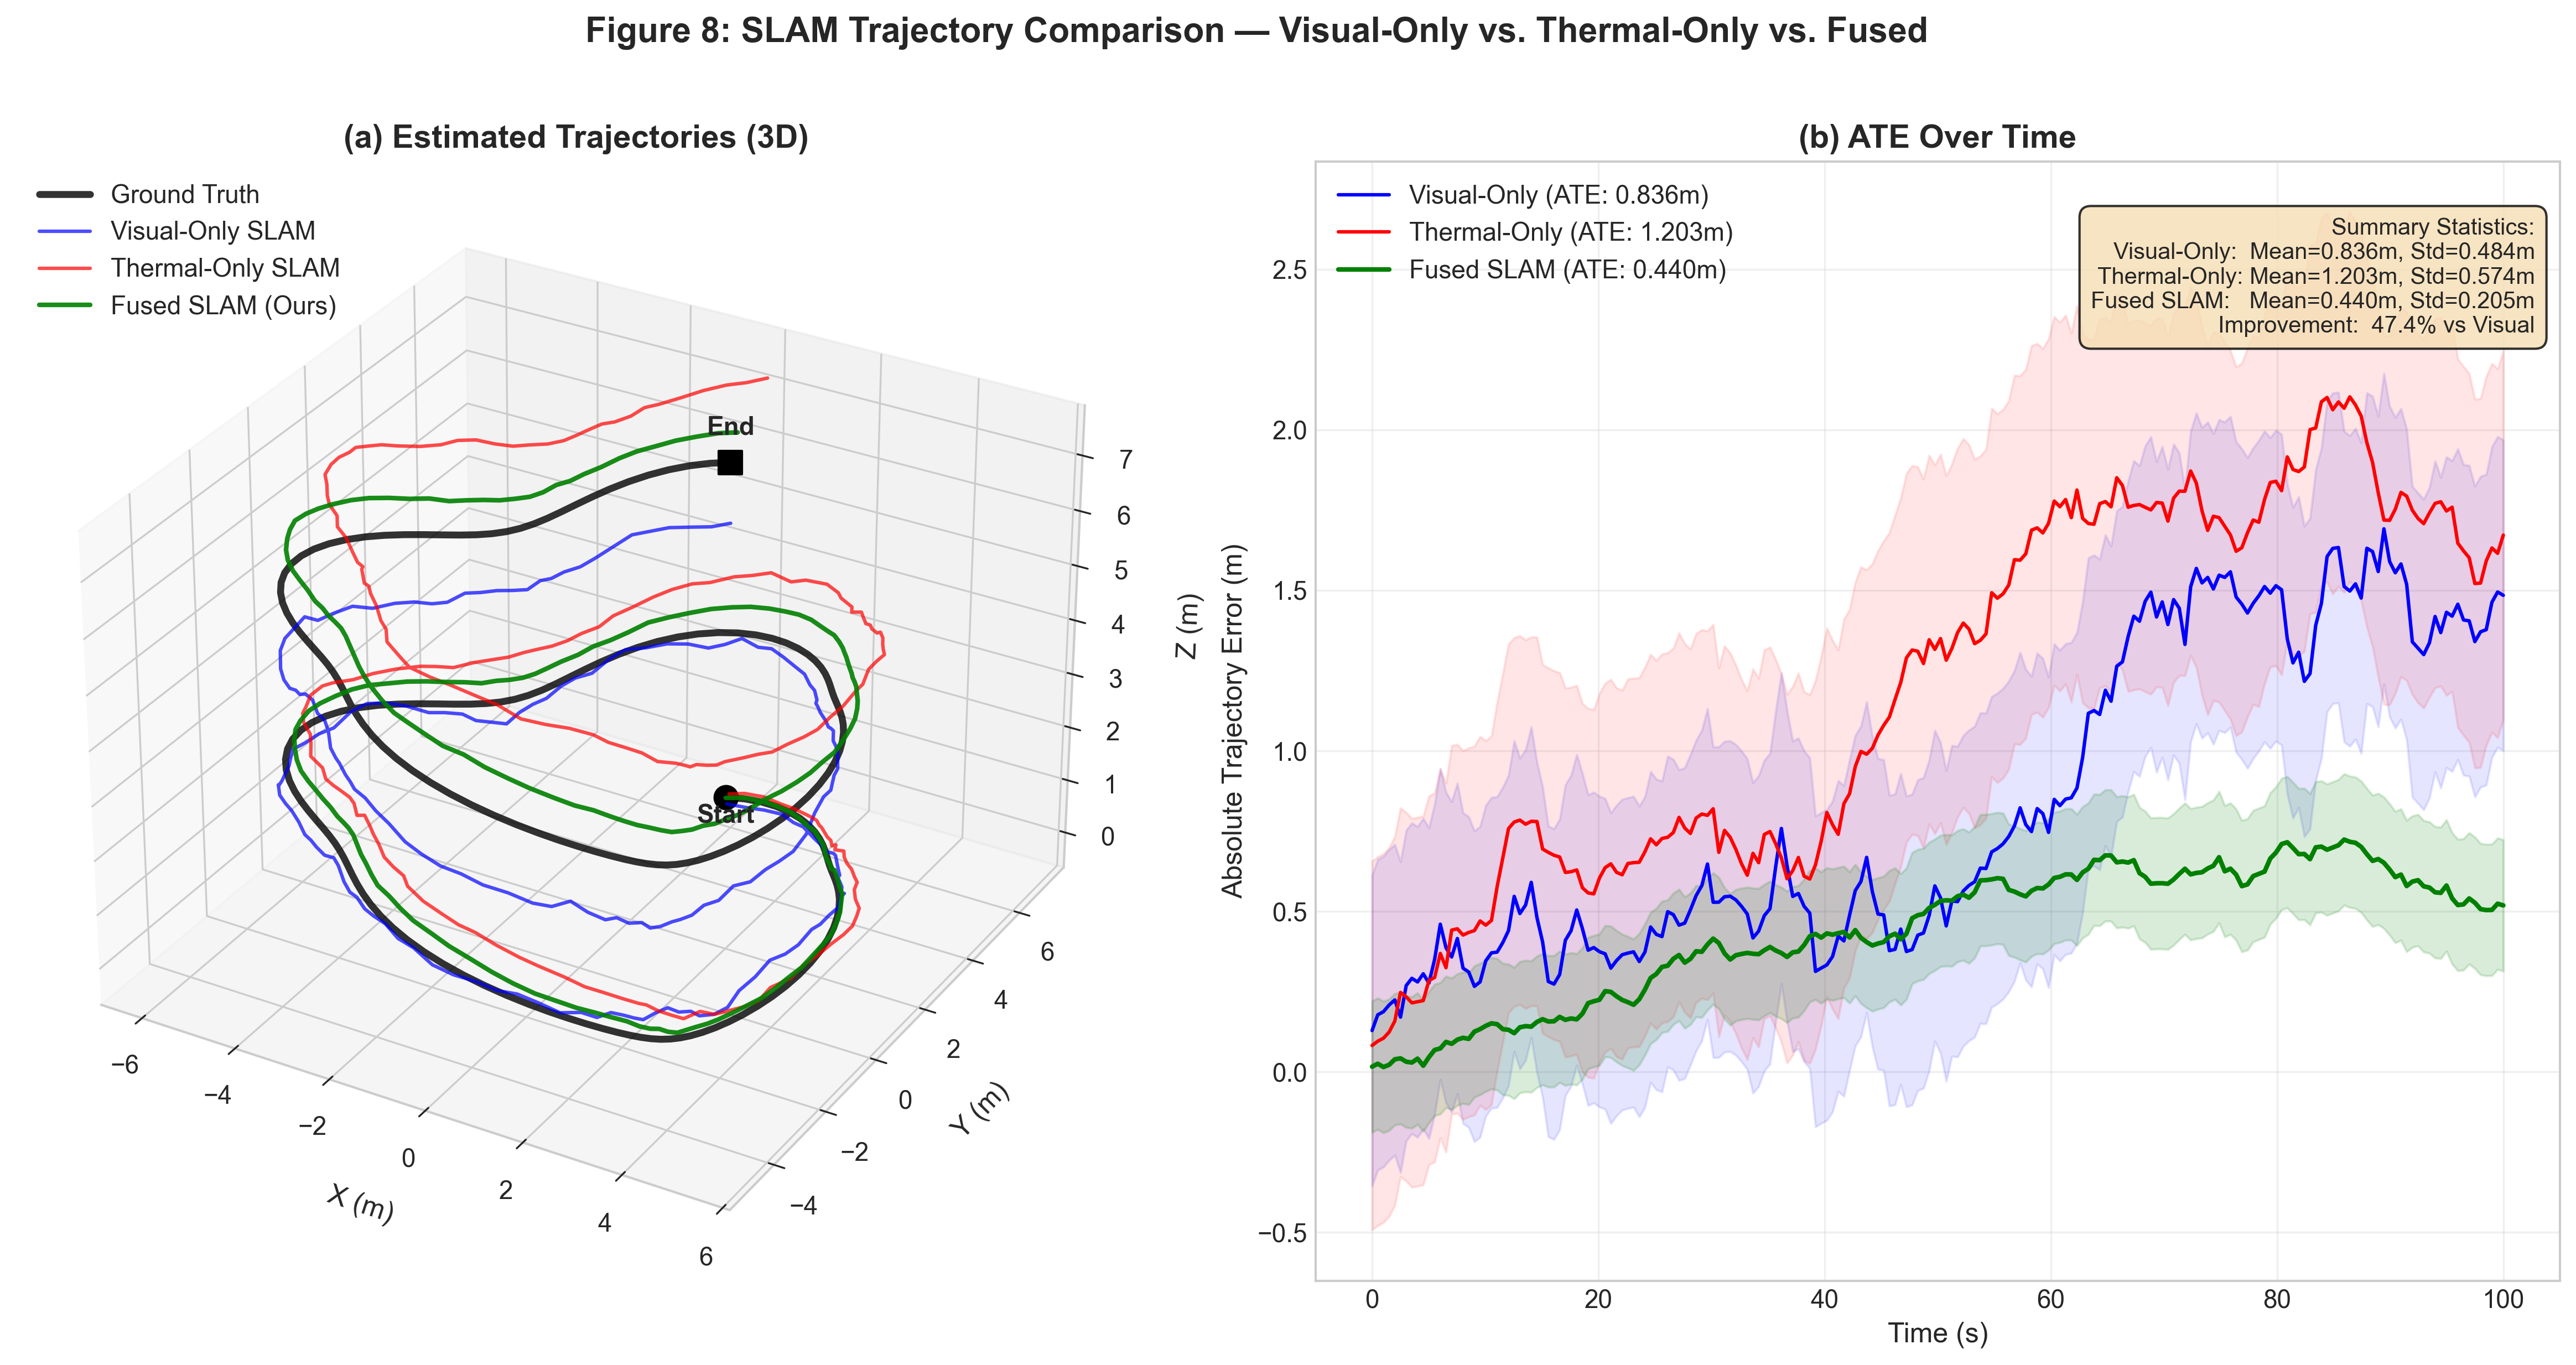
\includegraphics[width=\textwidth]{figures/fig_slam_trajectory_comparison.png}
\caption{השוואת מסלולי SLAM במסלול לילי: חזותי בלבד (אדום), תרמי בלבד (כחול), ממוזג (ירוק), ואמת קרקע (שחור). (SLAM trajectory comparison on a nocturnal path: visual-only (red), thermal-only (blue), fused (green), and ground truth (black).)}
\label{fig:ch04_slam_trajectory}
\end{figure*}

איור~\ref{fig:ch04_slam_trajectory} מציג השוואה ויזואלית של המסלולים המוערכים. ניתן לראות כי המסלול הממוזג (ירוק) קרוב ביותר לאמת הקרקע (שחור), בעוד שהמסלול החזותי בלבד (אדום) סובל מסחיפה משמעותית לאחר כ-200 מ' של נסיעה בתנאי חושך.

\subsection{סיכום}
\label{sec:ch04_summary}

בפרק זה הצגנו מסגרת \en{SLAM} היברידית המשלבת מידע ממצלמה תרמית ומצלמה חזותית. המסגרת מבוססת על ארכיטקטורת גרף-\en{SLAM} עם אופטימיזציית \en{pose graph}, תוך שימוש בשיטת התאמת נקודות עניין בין-מודאלית מבוססת למידה עמוקה ובאומדן עומק יחסי מתמונה תרמית יחידה. התוצאות מראות שיפור משמעותי בדיוק ובעמידות המערכת בתנאי תאורה נמוכה, עם שיעור הצלחה של 94\% בתנאי חושך מוחלט לעומת 15\% במערכת חזותית בלבד.